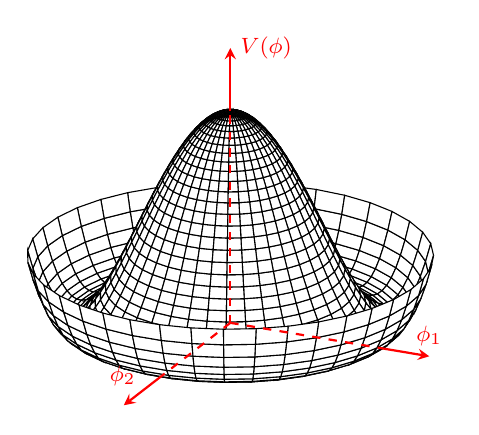
\begin{tikzpicture}

    \begin{axis}[
        %axis lines=center,
        %axis line style={->},
        hide axis,
        samples=40,
        domain=0:360,
        y domain=0:1.25,
        xtick=\empty,
        ytick=\empty,
        ztick=\empty
    ]
    \addplot3 [surf, shader=flat, draw=black, fill=white, z buffer=sort] ({sin(x)*y}, {cos(x)*y}, {(y^2-1)^2});

    \draw[red,thick,dashed] (axis cs:0,0,0) -- (axis cs:1,0,0)
                %node[below,font=\footnotesize]{$\phi_{1}$}
                ;
    \draw[red,thick,-stealth] (axis cs:1,0,0) -- (axis cs:1.35,0,0)
                node[above,font=\footnotesize]{$\phi_{1}$};

    \draw[red,thick,dashed] (axis cs:0,0,0) -- (axis cs:0,-1,0)
                node[left=2mm,font=\footnotesize]{$\phi_{2}$};
    \draw[red,thick,-stealth] (axis cs:0,-1,0) -- (axis cs:0,-1.55,0)
                %node[right=1mm,font=\footnotesize]{$\phi_{2}$}
                ;

    \draw[red,thick,dashed] (axis cs:0,0,0) -- (axis cs:0,0,1)
                %node[left=2mm,font=\footnotesize]{$\phi_{2}$}
                ;
    \draw[red,thick,-stealth] (axis cs:0,0,1) -- (axis cs:0,0,1.3)
                node[right,font=\footnotesize]{$V(\phi)$};

    \end{axis}

\end{tikzpicture}